%----------------------------------------------------------------------------------
% Exemplo do uso da classe tcc.cls. Veja o arquivo .cls
% para mais detalhes e instruções.
%----------------------------------------------------------------------------------

% Seleção de idioma da monografia. Por enquanto as únicas opções
% suportadas são 'portuguese' e 'english'
% Para impressão em frente e verso, use a opção 'twoside'. Da
% mesma forma, use 'oneside' para impressão em um lado apenas.
\documentclass[portuguese,oneside]{tcc}

%----------------------------------------------------------------
% Coloque seus pacotes abaixo.
%
% Obs.: muitos pacotes de uso comum do LaTeX, como amsmath,
% geometry e url já são automaticamente incluídos pela classe
% (veja o arquivo .cls). Isso torna obrigatória a presença destes
% no sistema para o uso desta classe, mas ao mesmo tempo o uso se
% torna mais simples.  Recomendo a instalação da versão mais
% recente da distribuição TeXLive (para Windows e UNIXes):
% www.tug.org/texlive/
%
% Pacotes e opções já incluídas automaticamente:
%
% \RequirePackage[T1]{fontenc}[2005/09/27]
% \RequirePackage[utf8x]{inputenc}[2008/03/30]
% \RequirePackage[english,brazil]{babel}[2008/07/06]
% \RequirePackage[a4paper]{geometry}[2010/09/12]
% \RequirePackage{textcomp}[2005/09/27]
% \RequirePackage{lmodern}[2009/10/30]
% \RequirePackage{indentfirst}[1995/11/23]
% \RequirePackage{setspace}[2000/12/01]
% \RequirePackage{textcase}[2004/10/07]
% \RequirePackage{float}[2001/11/08]
% \RequirePackage{amsmath}[2000/07/18]
% \RequirePackage{amssymb}[2009/06/22]
% \RequirePackage{amsfonts}[2009/06/22]
% \RequirePackage{url}
% \RequirePackage[table]{xcolor}[2007/01/21]
%----------------------------------------------------------------
% Para inserção de figuras.
\usepackage{graphicx}
% Utilize a opção 'pdftex' se você estiver usando o pdflatex (que
% permite figuras em formatos como .jpg ou .png)
%\usepackage[pdftex]{graphicx}

% Para tabelas com elementos ocupando mais de uma linha
\usepackage{multirow}
% Para frações na mesma linha (ex. ⅓).
\usepackage{nicefrac}
% Para inserir figuras lado a lado.
% \usepackage{subfigure}
% Para formatar algoritmos.
% A opção [algo2e] é necessária para evitar conflitos
% com as definições da classe.
%\usepackage[algo2e]{algorithm2e}
\usepackage{algorithmic}
% Um float do tipo algoritmo. No momento
% este pacote é incompatível com a classe.
%\usepackage{algorithm}

\usepackage{enumerate}
\usepackage{pgfgantt}
\usepackage{listings}

\definecolor{dkgreen}{rgb}{0,0.6,0}
\definecolor{gray}{rgb}{0.5,0.5,0.5}
\definecolor{mauve}{rgb}{0.58,0,0.82}

\lstset{frame=tb,
  aboveskip=3mm,
  belowskip=3mm,
  showstringspaces=false,
  columns=flexible,
  basicstyle={\small\ttfamily},
  numbers=none,
  numberstyle=\tiny\color{gray},
  keywordstyle=\color{blue},
  commentstyle=\color{dkgreen},
  stringstyle=\color{mauve},
  breaklines=true,
  breakatwhitespace=true,
  tabsize=3,
  language=python
}

\graphicspath{{images/}}

%----------------------------------------------------------------
% Autor (OBRIGATÓRIO)
%----------------------------------------------------------------
\author{Daniel Antoniazzi Amarante e Matthias Oliveira Nunes}

%----------------------------------------------------------------
% Título (OBRIGATÓRIO). Devem ser passados DOIS parâmetros,
% o título em português E o inglês, não importando o idioma
% escolhido. Os títulos são utilizados para a montagem da capa,
% resumo e abstract mais tarde.
%----------------------------------------------------------------
\title{Reconhecimento de Placas de Carro em um Sistema Embarcado}
      {Car License Plate Recognition in a Embedded System}

%----------------------------------------------------------------
% Opções para o tipo de trabalho (OBRIGATÓRIO)
%----------------------------------------------------------------
%\tipotrabalho{\ptci}         % Proposta de Trabalho de Conclusão
% \tipotrabalho{\tci}         % Trabalho de Conclusão I
\tipotrabalho{\tcii}        % Trabalho de Conclusão II

%----------------------------------------------------------------
% Seleção do curso ("este trabalho é um requisito parcial para
% obtenção do grau de (mestre ou doutor) em Ciência da Computação").
%----------------------------------------------------------------
\curso{\cc} % Ciência da Computação
%\curso{\si} % Sistemas de Informação
%\curso{\es} % Engenharia de Software

%----------------------------------------------------------------
% Orientador (e Co-orientador, caso haja um). É OBRIGATÓRIO
% informar pelo menos o orientador.
%----------------------------------------------------------------
\orientador{Roland Teodorowitsch}
%\coorientador{Ciclano de Farias}

%----------------------------------------------------------------
% A capa é inserida automaticamente. Por isso não é necessário
% chamar \maketitle
%----------------------------------------------------------------
\begin{document}

%----------------------------------------------------------------
% Depois da capa vem a dedicatória e a epígrafe.
%----------------------------------------------------------------
%\dedicatoria{Dedicamos este trabalho ao nosso amigo, Fernando Heck.}

%\epigrafe{Nice serve!}{Hinata Shoyo}

%----------------------------------------------------------------
% Também dá para fazer as duas na mesma página:
%----------------------------------------------------------------
%\dedigrafe{Dedico este trabalho a meus pais.}
%          {The art of simplicity is a puzzle of complexity.}
%          {Douglas Horton}

%----------------------------------------------------------------
% A seguir, a página de agradecimentos (OPCIONAL):
%----------------------------------------------------------------
%\begin{agradecimentos}
%À lorem ipsum, dolor sit amet consetetur sadipscing elitr sed diam
%nonumy eirmod tempor. Invidunt ut labore et dolore magna aliquyam

%À erad sed, diam voluptua at vero, eos et accusam et justo duo
%dolores et ea rebum stet clita.

%À kasd gubergren, no sea. Takimata sanctus est lorem ipsum dolor sit
%amet lorem ipsum dolor sit amet. Consetetur sadipscing elitr sed

%À diam nonumy, eirmod tempor, invidunt ut labore et dolore magna
%aliquyam erat sed diam voluptua at.
%\end{agradecimentos}

%----------------------------------------------------------------
% Resumo, com as palavras-chave passadas por parâmetro
% (OBRIGATÓRIO, ao menos para teses e dissertações)
%----------------------------------------------------------------
\begin{resumo}{Reconhecimento de placas de carro, Processamento de Imagens}
O controle e identificação de veículos é usado nas mais diversas áreas, indo
desde serviços de pagamentos automatizados, como pedágios, até aplicações
mais críticas, como segurança de fronteiras e sistemas de vigilância de
tráfego. Com o crescimento constante da frota de carros no Brasil,
aplicações para auxiliar neste trabalho tornam-se cada vez mais necessárias. O fato de que há peculiaridades nas placas automotivas brasileiras, que impossibilitam a utilização de ferramentas configuradas para placas estrangeiras, também evidencia a necessidade de soluções locais para este problema. Com isso em mente, propõe-se neste trabalho uma solução de aplicação embarcada de reconhecimento de placas.
\end{resumo}

%----------------------------------------------------------------
% Abstract, com as palavras-chave passadas por parâmetro
% (OBRIGATÓRIO, ao menos para teses e dissertações)
%----------------------------------------------------------------
\begin{abstract}{Automatic License Plate Recognition, Image Processing}
The identification and control of vehicles is used in many different areas, ranging from automated payment services, like toll booths, to more critical applications, such as border security and traffic vigilance systems. The fact that there are peculiarities in the brazilian license plates, that preclude the utilization of tools configured for international license plates, also points to the necessity of local solutions for that problem. With the constant growth of the Brazilian car fleet, applications used to help in this line of work become more necessary every day. With that in mind, it is proposed in this paper a solution of an embedded application for automatic license plate recognition. 
\end{abstract}

%----------------------------------------------------------------
% Listas e sumário, nessa ordem. Somente o sumário é obrigatório,
% portanto, comente as outras listas, caso sejam desnecessárias.
%----------------------------------------------------------------
\listoffigures       % Lista de figuras      (OPCIONAL)
%\listoftables        % Lista de tabelas      (OPCIONAL)
%\listofalgorithms    % Lista de algoritmos   (OPCIONAL)
%\listofacronyms      % Lista de siglas       (OPCIONAL)
%\listofabbreviations % Lista de abreviaturas (OPCIONAL)
%\listofsymbols       % Lista de símbolos     (OPCIONAL)
\tableofcontents     % Sumário               (OBRIGATÓRIO)

%----------------------------------------------------------------
% Aqui começa o desenvolvimento do trabalho. Para uma melhor
% organização do documento, separe-o em arquivos,
% um para cada capítulo. Para isso, utilize o comando \include,
% como mostrado abaixo.
%----------------------------------------------------------------
%\include{exemplo-cap1}
%\include{exemplo-cap2}
\chapter{Introdução}
\label{cha:intro}
O controle e identificação de veículos é usado nas mais diversas áreas, indo
desde serviços de pagamentos automatizados, como pedágios, até aplicações mais
críticas, como segurança de fronteiras, sistemas de vigilância de
tráfego~\cite{ahmad2015automatic} e sistema de busca por carros roubados.
Uma solução para identificar é, inclusive,  parte do plano de governo do atual prefeito eleito de Porto Alegre
Nelson Marchezan. Ele pretende utilizar os sistemas de controle de velocidade da cidade para também
monitorar as placas de carros com o objetivo de identificar carros roubados~\cite{psdb2016marchezan}.
Com o crescimento constante da frota de carros no Brasil, aplicações para
auxiliar neste trabalho tornam-se cada vez
mais nescessárias. Com isso em mente, propõe-se neste trabalho uma solução de
aplicação embarcada de reconhecimento de placas, visando a
crescente nescessidade de controle na área e as peculiaridades das placas
automotivas brasileiras, que nos impossibilitam de utilizar ferramentas
configuradas para placas estrangeiras, nescessitando pesquisas locais neste
tema.

O reconhecimento automático de placas de carros (\emph{Automatic License-Plate
Recognition}, ALPR) é a extração das informações das placas de veículos a partir
de uma imagem ou de uma sequência de imagens. A sua utilização na vida real
precisa de um processamento rápido e bem sucedido de placas sob diferentes
condições ambientais. Deve-se considerar as diferenças entre as placas de
diferentes nações, que terão cores, fontes, símbolos, padrões e línguas
diferentes. Também é preciso superar casos onde as placas possam estar
parcialmente cobertas com sujeira, luzes e acessórios dos
carros, e também a iluminação do ambiente e qualidade
da imagem adquirida.~\cite{s2013automatic}

A solução proposta neste trabalho tem como diferencial o fato de permitir uma
análise e processamento das imagens em tempo real. Isso será realizado
utilizando um software embarcado, que estará coletando as imagens ao mesmo tempo
que as analisa e as envia para um servidor. Com essa abordagem, será possível
que esses dados sejam úteis para uma tomada de decisão imediata do usuário.

Um exemplo de uma aplicação, onde a velocidade e a disponibilidade imediata das informações é
crucial para a viabilidade do produto, seria em um \emph{software} de identificação
de carros roubados. O sistema analisaria as placas dos carros que trafegam em uma
rodovia e identificaria quais daqueles carros tem placas que correspondem a placas
de carros roubados. Para que o \emph{software} seja eficiente é nescessário
que o processamento seja feito em tempo real, qualquer atraso na identificação do
veículo permite que ele se distancie muito, impedindo que as autoridades reajam a tempo.

Uma abordagem alternativa seria fazer a gravação das imagens em um momento, e o
processamento em outro. Entretanto, desta maneira, a utilidade do
\emph{software} seria limitada, pois na maioria das aplicações reais estes dados
precisam estar disponíveis imediatamente.

Com o resultado da implementação proposta será feita uma prova de conceito
utilizando o estacionamento da PUCRS, se for possível adquirir permissão.
Posicionando o computador com a câmera em um ponto estratégico do
estacionamento, serão analisados os carros que passarem. O programa então
coletará informações referentes ao número de carros que passaram por aquele ponto
e suas respectivas placas.

Este trabalho está organizado da seguinte maneira: No capítulo~\ref{cha:trab},
serão apresentados trabalhos relacionados aos temas de reconhecimento de placas
e contagem de carros. No capítulo~\ref{cha:modelo}, será apresentado o modelo
proposto. No capítulo~\ref{cha:implementacao}, será especificado os passos a serem
seguidos no desenvolvimento da aplicação, classificando os algoritmos a serem utilizados
em cada etapa. No capítulo~\ref{cha:configuracao}, será demonstrada como deve ser feita
a configuração e instalação das ferramentas nescessárias para o desenvolvimento do trabalho.
 E nos capítulos~\ref{cha:crono}  e~\ref{cha:recursos}, serão mostrados
o cronograma planejado e os recursos nescessários para a conclusão deste
trabalho respectivamente.


\chapter{Fundamentação Teórica}
\label{cha:fundamentacao}
Diversas técnicas e algoritmos são utilizadas nas aplicações de reconhecimento automático de placas de carros. Neste capítulo é feito um aprofundamento teórico sobre as técnicas utilizadas em todas as etapas do desenvolvimento do trabalho, explicando os principais algoritmos e conceitos aplicados na construção da ferramenta.

\section{Processamento de Imagens}
\label{sec:processamentoimagens}

Lorem ipsum dolor sit amet, consectetur adipiscing elit, sed do eiusmod tempor incididunt ut labore et dolore magna aliqua. Ut enim ad minim veniam, quis nostrud exercitation ullamco laboris nisi ut aliquip ex ea commodo consequat. Duis aute irure dolor in reprehenderit in voluptate velit esse cillum dolore eu fugiat nulla pariatur. Excepteur sint occaecat cupidatat non proident, sunt in culpa qui officia deserunt mollit anim id est laborum

\section{Reconhecimento Ótico de Caracteres}
\label{sec:ocr}

Reconhecimento Ótico de Caracteres (\emph{Optical Character Recognition}, OCR)
consiste da conversão de textos em formato de imagem para o formato reconhecido
por máquina. É o método mais eficiente para fazer o processamento de imagem para
texto de acordo com Mohit et al.~\cite{mohit2015designing}.

Uma ferramenta conhecida de OCR é o
\emph{Tesseract}\footnote{https://github.com/tesseract-ocr/tesseract}. É uma ferramenta
\emph{open source} de reconhecimento ótico de caracteres que suporta múltiplas
línguas.  É essencialmente um algoritmo de comparação de \emph{templates}, e as
amostras de caracteres podem ser auto-treinadas.~\cite{ho2016intelligent}

Neste trabalho, implementaremos um \emph{software} de reconhecimento ótico de caracteres focado especificamente em reconhecer caracteres de placas de transito brasileiras utilizando aprendizado de máquina com o algoritmo \emph{K-Nearest Neighbors} que será fundamentado na seção ~\ref{sec:knearest}

\section{Filtro Bilateral}
\label{sec:bilateralfilter}

Lorem ipsum dolor sit amet, consectetur adipiscing elit, sed do eiusmod tempor incididunt ut labore et dolore magna aliqua. Ut enim ad minim veniam, quis nostrud exercitation ullamco laboris nisi ut aliquip ex ea commodo consequat. Duis aute irure dolor in reprehenderit in voluptate velit esse cillum dolore eu fugiat nulla pariatur. Excepteur sint occaecat cupidatat non proident, sunt in culpa qui officia deserunt mollit anim id est laborum

\section{Detecção de Bordas}
\label{sec:detecbordas}

Detecção de bordas é um método de processamento de imagem desenvolvido para detectar pixels de borda. os pixels de borda são pixels em que a intensidade da imagem muda abruptamente, e as bordas são conjuntos de pixels de borda conexos.\cite{gonzalez1977digital}

\subsection{Filtro de Sobel}
\label{sec:sobel}

Lorem ipsum dolor sit amet, consectetur adipiscing elit, sed do eiusmod tempor incididunt ut labore et dolore magna aliqua. Ut enim ad minim veniam, quis nostrud exercitation ullamco laboris nisi ut aliquip ex ea commodo consequat. Duis aute irure dolor in reprehenderit in voluptate velit esse cillum dolore eu fugiat nulla pariatur. Excepteur sint occaecat cupidatat non proident, sunt in culpa qui officia deserunt mollit anim id est laborum

\section{Limiarização}
\label{sec:limiarizacao}

Lorem ipsum dolor sit amet, consectetur adipiscing elit, sed do eiusmod tempor incididunt ut labore et dolore magna aliqua. Ut enim ad minim veniam, quis nostrud exercitation ullamco laboris nisi ut aliquip ex ea commodo consequat. Duis aute irure dolor in reprehenderit in voluptate velit esse cillum dolore eu fugiat nulla pariatur. Excepteur sint occaecat cupidatat non proident, sunt in culpa qui officia deserunt mollit anim id est laborum

\subsection{Método de Otsu}
\label{sec:otsu}

Lorem ipsum dolor sit amet, consectetur adipiscing elit, sed do eiusmod tempor incididunt ut labore et dolore magna aliqua. Ut enim ad minim veniam, quis nostrud exercitation ullamco laboris nisi ut aliquip ex ea commodo consequat. Duis aute irure dolor in reprehenderit in voluptate velit esse cillum dolore eu fugiat nulla pariatur. Excepteur sint occaecat cupidatat non proident, sunt in culpa qui officia deserunt mollit anim id est laborum

\section{Operações Morfológicas}
\label{sec:morfologicas}

Lorem ipsum dolor sit amet, consectetur adipiscing elit, sed do eiusmod tempor incididunt ut labore et dolore magna aliqua. Ut enim ad minim veniam, quis nostrud exercitation ullamco laboris nisi ut aliquip ex ea commodo consequat. Duis aute irure dolor in reprehenderit in voluptate velit esse cillum dolore eu fugiat nulla pariatur. Excepteur sint occaecat cupidatat non proident, sunt in culpa qui officia deserunt mollit anim id est laborum

\subsection{Erosão}
\label{sec:erosao}

Lorem ipsum dolor sit amet, consectetur adipiscing elit, sed do eiusmod tempor incididunt ut labore et dolore magna aliqua. Ut enim ad minim veniam, quis nostrud exercitation ullamco laboris nisi ut aliquip ex ea commodo consequat. Duis aute irure dolor in reprehenderit in voluptate velit esse cillum dolore eu fugiat nulla pariatur. Excepteur sint occaecat cupidatat non proident, sunt in culpa qui officia deserunt mollit anim id est laborum

\subsection{Dilatação}
\label{sec:dilatacao}

Lorem ipsum dolor sit amet, consectetur adipiscing elit, sed do eiusmod tempor incididunt ut labore et dolore magna aliqua. Ut enim ad minim veniam, quis nostrud exercitation ullamco laboris nisi ut aliquip ex ea commodo consequat. Duis aute irure dolor in reprehenderit in voluptate velit esse cillum dolore eu fugiat nulla pariatur. Excepteur sint occaecat cupidatat non proident, sunt in culpa qui officia deserunt mollit anim id est laborum

\subsection{Abertura}
\label{sec:abertura}

Lorem ipsum dolor sit amet, consectetur adipiscing elit, sed do eiusmod tempor incididunt ut labore et dolore magna aliqua. Ut enim ad minim veniam, quis nostrud exercitation ullamco laboris nisi ut aliquip ex ea commodo consequat. Duis aute irure dolor in reprehenderit in voluptate velit esse cillum dolore eu fugiat nulla pariatur. Excepteur sint occaecat cupidatat non proident, sunt in culpa qui officia deserunt mollit anim id est laborum

\subsection{Fechamento}
\label{sec:fechamento}

Lorem ipsum dolor sit amet, consectetur adipiscing elit, sed do eiusmod tempor incididunt ut labore et dolore magna aliqua. Ut enim ad minim veniam, quis nostrud exercitation ullamco laboris nisi ut aliquip ex ea commodo consequat. Duis aute irure dolor in reprehenderit in voluptate velit esse cillum dolore eu fugiat nulla pariatur. Excepteur sint occaecat cupidatat non proident, sunt in culpa qui officia deserunt mollit anim id est laborum

\section{K-Nearest Neighbors}
\label{sec:knearest}

\emph{K-Nearest Neighbors} é um dos mais simples algoritmos de classificação disponíveis para aprendizado supervisionado em aprendizado de máquina.~\cite{opencv2014knearest} Aprendizado supervisionado é tarefa de inferir uma função a partir de dados de treinamento rotulados. O algoritmo recebe um conjunto de exemplos como dados de treinamento e faz predições para os pontos não vistos com base nestes dados.~\cite{mohri2012foundations} A ideia do algoritmo \emph{K-Nearest Neighbors} é encontrar a combinação mais próxima de um determinado dado de teste em um espaço de dados.~\cite{opencv2014knearest}

\begin{figure}[H]
	\centering
	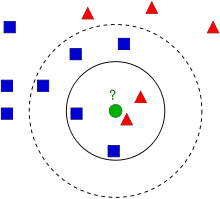
\includegraphics[width=50mm]{knn_theory.png}
	\caption{Exemplo de aplicação do K-Nearest Neighbors}
Fonte: Understanding k-Nearest Neighbour~\cite{opencv2014knearest}
	\label{fig:knearest_example}
\end{figure}

Em um caso hipotético de aplicação do algoritmo existem duas classes, a classe dos quadrados azuis e a classe dos triângulos vermelhos. Este exemplo está ilustrado na figura \ref{fig:knearest_example}. Pontos representando estas classes são espalhados em um espaço chamado de \emph{feature space}. Estes espaços são os espaços onde todos os dados estão projetados. Em um espaço de duas dimensões, como no exemplo, cada dado tem duas características, x e y. Em um espaço de três dimensões, cada dado teria 3 característica, em N dimensões, N características.

Na adição de um novo dado no \emph{feature space}, ele deve ser classificado como uma das duas classes. Este é o chamado de processo de classificação, onde o algoritmo é aplicado.

Um método é o de calcular quem é o vizinho mais próximo. Na imagem, este seria o triangulo vermelho. Este método é chamado de \emph{Nearest Neighbor}, ou o vizinho mais próximo, pois a classificação só depende de um vizinho.

Outro método seria checar múltiplos vizinhos para ver quantos vizinhos de cada classe o novo dado possui. Na imagem, o triangulo vermelho é o vizinho mais próximo, mas, considerando múltiplos vizinhos, é possível classificar o novo dado na classe dos quadrados azuis, pois existem mais vizinhos desta classe. Este método é chamado de \emph{k Nearest Neighbors}, pois ele considera uma quantidade pré determinada \emph{k} de vizinhos para classificar seus novos dados. ~\cite{opencv2014knearest}

Neste projeto o algoritmo \emph{K-Nearest Neighbors} é utilizado na implementação do reconhecedor ótico de caracteres encontrados em placas de transito brasileiras. São utilizados como dados de teste as letras maiúsculas e números na fonte \emph{Mandatory}, e são aproximados os valores dos caracteres segmentados da placa com base nestes. Como teremos apenas um valor para cada classe, cada classe representando um caractere diferente, utilizaremos apenas o vizinho mais próximo para classificar nossos caracteres. Tendo um conjunto de treinamento maior, é possível aumentar este valor.
 

\chapter{Trabalhos Relacionados}
\label{cha:trab}
Uma solução para detectar e reconhecer placas de licenciamento brasileiras foi
proposta por Serro~\cite{serro2012deteccao} na PUCRS\@. Neste trabalho foram
utilizadas técnicas de segmentação de imagens, histograma, cisalhamento de
imagens e reconhecimento ótico de caracteres. A metodologia utilizada consistiu das
seguintes etapas, calibração do sistema
para definir a região de interesse e o ângulo de cisalhamento, detecção da
placa, segmentação dos caracteres e aplicação do reconhecedor ótico de
caracteres.

Com a solução proposta por Serro~\cite{serro2012deteccao}  foi obtida uma taxa de
acerto de aproximadamente 54\%, com tempo médio de execução de 0,062 segundos por imagem.
A baixa taxa de acerto pode ter sido por problemas de foco e nitidez, o tamanho da placa em
\emph{pixels} nas imagens e a existência de outros objetos em cena. Todos esses
problemas foram citados no desenvolvimento do projeto.

Em Ahmad et al.~\cite{ahmad2015automatic} foi feito um estudo comparativo dos
sistemas de reconhecimento de placas automotivas automáticos. Segundo estes
autores, o processo de ler o conteúdo de uma placa passa por três estágios. O
primeiro é a localização ou extração da placa, que consiste no processo de
localizar a placa do carro na imagem. O segundo estágio é a separação dos
caracteres, onde cada caractere individual é separado dos outros para
reconhecimento. E o terceiro e último estágio é o reconhecimento do caractere em
si, onde os caracteres extraídos da imagem são identificados.

Neste trabalho foram implementados três diferentes métodos de localização de
placa e dois diferentes métodos de reconhecimento de caracteres, resultando em 6
diferentes abordagens para o reconhecimento de placas. Todas essas combinações
foram então testadas contra diferentes conjuntos de dados.

Os resultados obtidos por Ahmad et al.~\cite{ahmad2015automatic} na experimentação não
foram muito animadores, variando entre 20 e 40 por cento.
Um dos motivos para os maus resultados foi a variedade de parâmetros nas imagens do conjunto
de dados de teste. Tais parâmetros incluem
variações na distância, ângulo, iluminação e ambiente. Estes erros poderiam ser
mitigados em sistemas reais com uma câmera com resolução fixa e de boa
qualidade. A variação do tamanho da placa afetou o desempenho de alguns
algoritmos, mas em uma câmera fixa é possível obter uma consistência e conseguir
resultados mais aceitáveis.

Outros motivos para a baixa taxa de acerto foram a falta de pré-processamento
das imagens, que a análise não considerou, e a utilização de mais dados de
aprendizado para o reconhecimento ótico de caracteres.

Em Abtahi et al.~\cite{abtahi2015deep} foram feitas novas abordagens para a
segmentação de caracteres em imagens. De acordo com eles, o método padrão de
segmentação baseado em projeção sofre com variações consideráveis na região da
placa ao redor dos caracteres, portanto estes autores propuseram duas abordagens.
A primeira é feita adaptando um método de aprendizado por reforço, criando um agente que
consiga achar os melhores caminhos para a segmentação.  A segunda abordagem usa
um método híbrido que utiliza a simplicidade e velocidade do método de projeção,
mas com o poder do aprendizado por reforço.

De acordo com Wafy e Madbouly~\cite{wafy2016efficient}, o reconhecimento de uma
placa consiste em dois mecanismos principais: detecção de uma placa e em seguida
a sua identificação. O algoritmo proposto nesse artigo, faz os dois passos e se
baseia na distribuição semi-simétrica dos pontos de canto nas imagens de carros
e placas, e nas características morfológicas da região da placa. Essa solução
teve uma taxa de acerto de 97,5\% no processo de detecção e 92,8\% na
identificação, com o maior tempo de execução para um dos processos sendo de
0,3s. Com estes resultados seria possível utilizar este método em aplicações de
tempo real.

Com relação ao uso de sistema embarcado para executar o reconhecimento, Arth et
al.~\cite{arth2007real} trabalharam no desenvolvimento de um sistema de reconhecimento
de placas de carro em um processador de digital de sinal (\emph{Digital Signal Processor}, DSP).
\emph{DSP} são microprocessadores especializados em processamento digital de sinal utilizados para
processar sinais como áudio ou vídeo em tempo real.~\cite{yovits1993advances} O processador utilizado
neste trabalho específico foi um \emph{Texas Instruments C64} com \emph{1MB} de \emph{cache RAM} e um outro bloco
de memória mais lento, \emph{SDRAM} de \emph{16MB}. O processador não possui camera integrada mas permite a conexão de
uma fonte de vídeo analógica ou digital. Na solução implementada foi utilizada uma camera com resolução de \emph{352x288 pixels}.

Com sua implementação, Arth et al.~\cite{arth2007real} foram capazes de conseguir localizar a placa em
\emph{7.30 ms}, levando mais aproximadamente \emph{1 ms} para identificar cada caractere. Não é informado no artigo
a taxa de sucesso de cada reconhecimento. Os autores ainda concluem que por o tempo de detecção da placa ser superior
ao tempo de reconhecimento dos caracteres, este algoritmo deve ser melhorado.

Analisando os trabalhos feitos na área, nota-se que por mais que os algoritmos variem,
a base da detecção de placas permanece parecida. Eles costumam ser divididos em pelo
menos duas partes, a localização da placa e a detecção dos caracteres. Inclusive~\cite{ahmad2015automatic}
misturou diferentes algoritmos, utilizando a localização de um e a detecção de
outro, demonstrando que os dois passos são bem independentes.

Pode-se notar que o reconhecimento de placas de carros é uma área bastante estudada,
com diversas abordagens diferentes e grande variação de resultados. Entretanto,
um problema que ainda existe, é a grande diferença nas placas de diferentes países,
no estilo, fonte, caracteres utilizados e padrão do texto.

O \emph{software open source Openalpr}\footnote{https://github.com/openalpr/openalpr}
criou uma solução de reconhecimento de placas que permite que a comunidade contribua
treinando o reconhecedor de caracteres a reconhecer as placas de seus países para contornar
esse problema.


\chapter{Ambiente de Desenvolvimento}
\label{cha:componentes}
Para o desenvolvimento do trabalho serão utilizados alguns componentes externos,
tanto de \emph{hardware} quanto de \emph{software}. Será utilizado o computador
\emph{Raspberry Pi} e seu módulo de camera. Será utilizada a linguagem de programação
\emph{Python}. Será utilizada a biblioteca de visão computacional \emph{OpenCV}
juntamente com outras bibliotecas auxiliares que permitam integrar o \emph{OpenCV}
com a linguagem de programação \emph{Python} e o módulo de camera do \emph{Raspberry Pi}.

\section{Raspberry Pi}
\label{sec:raspi}

\begin{figure}[H]
	\centering
	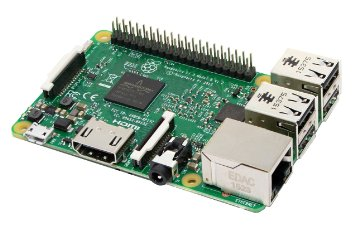
\includegraphics[width=88mm]{raspberrypi.jpg}
	\caption{O Raspberry Pi 3 model B}
	\label{fig:raspberrypi}
\end{figure}

Raspberry Pi é um computador construído em uma placa de circuito do tamanho de
um cartão de crédito desenvolvido pela Raspberry Pi
Foundation\footnote{https://www.raspberrypi.org/}. Existem diversos modelos
diferentes de Raspberry Pi no mercado, o que será utilizado no trabalho é um dos
mais recentes, o Raspberry Pi 3 model B. Será utilizado o sistema
operacional \emph{Raspbian}, que é o sistema operacional oficial suportado pela
\emph{Raspberry Pi Foundation}.

O computador ainda tem suas limitações, com um processador
quad-core ARMv8 de 1.2GHz e apenas 1GB de memória RAM\@. Pela limitação do
\emph{hardware} é possível que algumas aplicações fiquem mais lentas do que
ficariam em um computador mais potente, apesar disso, o Raspberry Pi é um
computador bem completo e capaz de exercer todas as funções de um computador
normal.

O modelo utilizado de Raspberry Pi contém módulo de WiFi embutido, sem a
nescessidade de periférico, que será utilizado no trabalho para enviar as
informações processadas pela Internet. Também será utilizado um módulo externo
de câmera para coletar as imagens em tempo real.

\section{OpenCV}
\label{sec:opencv}

OpenCV (\emph{Open Source Computer Vision Library}) é uma biblioteca \emph{open
source} de visão computacional e aprendizado de máquina. Contém mais de 2500
algoritmos otimizados nessas áreas, incluindo algoritmos clássicos e recentes. A
biblioteca é escrita nativamente em C++, e dispõe de interfaces para C, C++,
Python, Java e MATLAB, suportando os sistemas operacionais Windows, Linux,
Android e Mac OS.\footnote{http://opencv.org/}

No desenvolvimento deste trabalho será utilizada a linguagem de programação \emph{Python},
e algumas bibliotecas são utilizadas para trabalhar com \emph{OpenCV}. A biblioteca
\emph{numpy}\footnote{http://www.numpy.org/}, é uma biblioteca de computação científica em
\emph{Python}, que inclui funções de processamento numérico e vetores que são utilizados pelo \emph{OpenCV} para representar as imagens. 

Para as aplicações de aprendizado de máquina será utilizada a biblioteca \emph{ml} que é um módulo do \emph{OpenCV}. Esta biblioteca contém um conjunto de classes e métodos para classificação estatística, regressão e agrupamento de dados.\footnote{http://docs.opencv.org/2.4/modules/ml/doc/ml.html}

Também será utilizada o pacote \emph{picamera}\footnote{https://picamera.readthedocs.io/en/release-1.12/},
que possui uma interface em \emph{Python} para se comunicar com o módulo de camera do \emph{Raspberry Pi}.
É possível utilizar as funções próprias de captura de imagem da camera do \emph{OpenCV}, como por exemplo
o \texttt{cv2.VideoCapture(0)}, mas será optado por utilizar o \emph{picamera}, por ser uma interface mais
específica para a camera utilizada.


\chapter{Solução Desenvolvida}
\label{cha:implementacao}
Segundo Ahmad et al.~\cite{ahmad2015automatic}, o reconhecimento de placas
automotivas requer três passos, a localização da placa, a separação dos
caracteres e o reconhecimento dos caracteres.~\cite{s2013automatic} ainda defende 
que são nescessários os mesmos passos, com a inclusão da aquisição das imagens como passo inicial. 
Para a localização da placa e
separação dos caracteres serão utilizados a biblioteca OpenCV e a linguagem de
programação C, C++ ou Python. O motivo da escolha dessas linguagens se dá porque
são as linguagens mais usadas para OpenCV, a melhor abordagem ainda será
analisada. Para o reconhecimento dos caracteres será utilizado o software Tesseract, havendo a 
possibilidade de precisar ser treinado para reconhecer a fonte da placa de transito brasileira. As escolhas a serem
feitas tem como objetivo maximizar os resultados ao final do trabalho, tentando
criar um balanço entre facilidade de implementação e qualidade do
reconhecimento.

\section{Segmentação}
\label{sec:segmentacao}

O terceiro passo para o reconhecimento da placa é a segmentação dos caracteres. A segmentação dos caracteres 
consiste na extração dos caracteres utilizando estratégias como projetar as suas informações de cores, rotulá-los 
ou comparar suas posições com modelos. A placa extraida no passo anterior pode conter problemas de inclinação ou 
iluminação, mas o algoritmo de segmentação deve superar todos esses problemas com preprocessamento. ~\cite{s2013automatic}

~\cite{s2013automatic} faz uma análise dos algoritmos de segmentação mais utilizados com seus prós e contras. 
Os principais algoritmos utilizados são: segmentação utilizando conectividade de pixels, segmentação utilizando perfis 
de projeção, segmentação utilizando conhecimento anterior dos caracteres, segmentação utilizando contorno dos caracteres 
e segmentação utilizando características combinadas.

Analisando os resultados foi definido que a segmentação dos caracteres utilizando perfis de projeção foi o mais eficiente,
e que mais se encaixa no problema proposto.~\cite{sanyuan2004car} utiliza essa técnica de segmentação de caracteres, e, 
utilizando-a juntamente de remoção de ruidos e análise de sequencia de caracateres,obteve uma taxa de acerto de 99.2\% e 
uma velocidade de processamento de 10 a 20 milisegundos, o que é bem animador. As vantagens deste método é que a segmentação 
independe das posições dos caracteres, e consegue lidar bem com rotações. Suas desvantagens são que é afetada ruído na imagem 
e requer o conhecimento do número de caracteres na placa, o que não será problema devido ao fato de as placas brasileiras terem 
um número constante de caracteres.

Este método utiliza-se da diferença entre a cor dos caracteres da placa e a cor do fundo da placa, por terem valores diferentes 
eles tem valores binários opostos em uma imagem binária. Portanto, o método de segmentação consiste em projetar a placa extraída 
verticalmente para determinar o inicio e final dos caracteres e depois projetar os caracteres extraídos horizontalmente para extraír 
cada caracter independente.

~\cite{s2013automatic} ainda afirma que é evidente que este metodo de segmentação é o mais comum e o mais simples presente na 
literatura.


\chapter{Resultados Obtidos}
\label{cha:resultados}
Para a análise da solução desenvolvida e identificação de problemas foram feitos
testes variados. Este capítulo foi dividido em seções que representam as
descobertas mais relevantes ao longo da pesquisa e desenvolvimento. A
seção~\ref{sec:extracao_da_placa_resultados} vai descrever os resultados obtidos
na experimentação com a extração da placa nas imagens, a
seção~\ref{sec:reconhecimento_dos_caracteres_resultados} vai abordar os
resultados obtidos no reconhecimento dos caracteres e a
seção~\ref{sec:performance_resultados} vai abordar como performa o algoritmo no
computador \emph{Raspberry Pi}.

Foram coletadas imagens de 48 veículos distintos para analisar a capacidade de
reconhecimento do sistema. A tabela~\ref{tab:resultados} mostra o número de
imagens processadas, o número de imagens onde a placa foi encontrada com sucesso
e o número de imagens onde foi possível reconhecer o valor da placa.

\begin{table}[]
\centering
\caption{Resultados obtidos}
\label{tab:resultados}
\begin{tabular}{@{}lr@{}}
\toprule
Placas                               & \multicolumn{1}{l}{Resultado} \\ \midrule
Total de Imagens                     & 48                           \\
Imagens onde a placa foi encontrada  & 22                            \\
Imagens onde a placa foi reconhecida & 19
\end{tabular}
\end{table}

\section{Extração da placa}
\label{sec:extracao_da_placa_resultados}

Das 48 imagens adquiridas, apenas em 22 imagens foi possível extrair a placa. Dessas 48 imagens, 27 foram adquiridas ao ar livre, durante o dia e 21 foram adquiridas em local fechado, com iluminação baixa. Com essa diferença foi possível analisar o sistema nos dois tipos diferentes de ambientes. Nas imagens ao ar livre, com boa iluminação, houve um percentual de 55\% de acerto, enquanto nas imagens em ambiente fechado, com baixa iluminação, houve um percentual de acerto de 33\%. Os resultados comparativos podem ser vistos na Tabela~\ref{tab:resultados_ambientes}. Os exemplos são poucos para tirar conclusões, mas indicam que existe mais dificuldade para reconhecer placas em imagens mais escuras.

\begin{table}[]
\centering
\caption{Resultados obtidos em diferentes ambientes}
\label{tab:resultados_ambientes}
\begin{tabular}{@{}lr@{}}
\toprule
placas                                      		& \multicolumn{1}{l}{Resultado} \\ \midrule
Imagens ao ar livre com boa iluminação     			& 27                            \\
Total de acertos com boa iluminação    			 	& 15                            \\
Percentual de acertos com boa iluminação    		 & 55\%                            \\
Imagens em ambiente fechado com baixa iluminação     & 21                            \\
Total de acertos com baixa iluminação    			 & 7                            \\
Percentual de acertos com baixa iluminação 			& 33\%
\end{tabular}
\end{table}

O algoritmo de extração da placa é limitado com relação a distância que o carro
está na imagem. Na etapa de abertura e fechamento morfológicos, que tem o
objetivo de detectar as áreas de placas candidatas, o tamanho do elemento
estruturante influencia diretamente a qualidade da extração. Se utilizado um
elemento estruturante muito grande, é possível que na etapa de abertura, a placa
seja erodida junto com o ruído. Se utilizado um elemento estruturante muito
pequeno, muitas regiões sobram, diminuindo a performance do reconhecimento.

Colocar aqui imagem de exemplo mostrando a placa sendo destruída

\section{Reconhecimento dos caracteres}
\label{sec:reconhecimento_dos_caracteres_resultados}

Inicialmente foi utilizado o \emph{software Tesseract} para fazer o
reconhecimento dos caracteres, mas os resultados utilizando a ferramenta pura
não foram bons. Mesmo limitando os caracteres possíveis, informando ao
\emph{software} se o caractere seria um número ou uma letra, ainda havia
dificuldade no reconhecimento. Mesmo caracteres que não são tão semelhantes,
como o 5 e o 6, o \emph{software} não conseguiu distinguir.

Com a substituição do reconhecedor de caracteres \emph{Tesseract} para o
implementado com o algoritmo \emph{K-Nearest Neighbors} os resultados foram bem
melhores, obtendo sucesso no reconhecimento de 86\% das placas extraídas. Até
mesmo em imagens de placas inclinadas, como é o caso da
Figura~\ref{fig:plate_torta_result}, foi possível identificar os caracteres.

\begin{figure}[H]
	\centering
	
\includegraphics[width=88mm]{a42fill_binary_results.jpg}
	\caption{Placa inclinada que o sistema foi capaz de identificar}
	\label{fig:plate_torta_result}
\end{figure}

Das 22 placas extraídas, em três casos o reconhecedor de caracteres não teve
capacidade de ler. Dois destes foram causados por problemas na imagem e o outro
foi causado por semelhança de caracteres.

Placas com reflexo causado pelo ambiente, como a luz solar, podem impactar no
reconhecimento. O sol refletido no caractere da imagem pode dificultar o
processo de limiarização. Neste processo, ao diferenciar os caracteres escuros
do fundo cinza, a cor do caractere na imagem fica mais clara, sendo ele
parcialmente confundido com fundo. Na figura~\ref{fig:cagado_reflexo} é possível
observar uma placa que o reflexo impediu o reconhecimento correto.

\begin{figure}[H]
	\centering
	
\includegraphics[width=88mm]{3cagado.jpg}
	\caption{Placa com caractere mal reconhecido por causa de reflexo}
	\label{fig:cagado_reflexo}
\end{figure}

Placas desgastadas, pelo tempo ou pelo carro ter passado por condições climáticas que o degradaram, também não foram possível reconhecer corretamente. Assim como no caso anterior, os caracteres ficaram desfigurados na fase da limiarização, por terem uma variação muito grande nos tons de cinza. Isso faz com que parte do caractere seja confundido com o fundo. Imagem de placa de carro adquirida onde a placa estava desgastada dificultando o reconhecimento pode ser vista na Figura~\ref{fig:placa_desgastada}.

\begin{figure}[H]
	\centering
	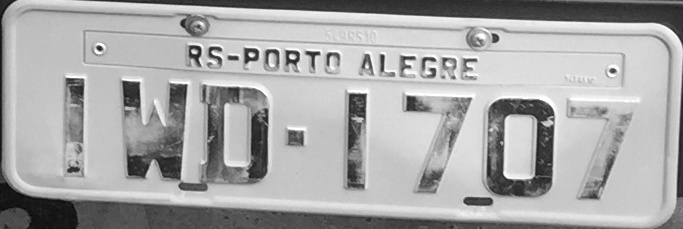
\includegraphics[width=88mm]{plca_desgastada.jpg}
	\caption{Placa desgastada}
	\label{fig:placa_desgastada}
\end{figure}

Somente em um caso, nas imagens de teste adquiridas, ocorreu um erro de reconhecimento de caractere por motivos não causados pelo ambiente ou qualidade da placa. Em uma imagem adquirida com a placa levemente inclinada, houve confusão, por parte do algoritmo, entre os caracteres "O" e "Q". Estes caracteres já são bastante semelhantes por si só, mas é possível, também, que o fato de a placa estar inclinada tenha amplificado o erro. A imagem que não foi reconhecida corretamente, ao confundir o "O" e o "Q" pode ser vista na Figura~\ref{fig:q_confundido_com_o}.

\begin{figure}[H]
	\centering
	
\includegraphics[width=88mm]{q_confundido_com_o.jpg}
	\caption{Placa que confundiu os caracteres O e Q}
	\label{fig:q_confundido_com_o}
\end{figure}

Apesar dos casos em que houve erro, o resultado do reconhecedor de caracteres foi satisfatório. Mesmo tendo sido sido utilizados apenas um exemplo para cada caractere, somente em um caso houve confusão no reconhecimento dos caracteres bem segmentados. Com mais exemplos seria possível um reconhecimento ainda mais preciso, mas essa etapa não é a etapa com mais problemas do projeto, não sendo prioridade para aperfeiçoar.

\section{Performance em sistema embarcado}
\label{sec:performance_resultados}

Dado o fato de a solução desenvolvida ser dividida em etapas, é possível avaliar
quais os passos levam mais tempo para serem executados, que podem ser
considerados os gargalos da aplicação. Em uma visão mais ampla, fica claro que a
etapa de extração da placa é a que necessita de mais recursos computacionais.
Isso se dá principalmente por ter que processar uma imagem maior que a imagem da
placa. O tempo utilizado para processar a placa extraída é, relativamente, bem
menor.

Para melhor analisar os resultados comparativos, foram calculadas as médias de
tempo de execução de cada etapa em múltiplas imagens e calculados seus valores
percentuais em relação ao tempo total de processamento de uma placa. Esses
valores independem do \emph{hardware} utilizado e do tamanho de imagem
utilizado, permitindo uma visão diferente dos resultados. Os resultados
comparativos podem ser vistos na Tabela~\ref{tab:resultados_relativos}.

\begin{table}[H]
\centering
\caption{Resultados relativos da fase de extração}
\label{tab:resultados_relativos}
\begin{tabular}{@{}lr@{}}
\toprule
Etapa                        & Tempo Percentual \\ \midrule
Conversão para tons de cinza & 10\%             \\
Filtro Bilateral             & 10\%             \\
Equalização do Histograma    & 10\%             \\
Limiarização                 & 10\%             \\
Detecção de Bordas           & 10\%             \\
Dilatação                    & 10\%             \\
Preenchimento de espaços     & 10\%             \\
Abertura                     & 10\%             \\
Fechamento                   & 10\%             \\
Extração das Regiões         & 10\%             \\ \bottomrule
\end{tabular}
\end{table}

A primeira implementação do algoritmo teve maus resultados com relação a
performance.

Falar sobre os resultados aqui.

Para tentar aprimorar a velocidade do processamento em imagens consecutivas foi
aplicado o uso de múltiplos processos, com o objetivo de utilizar todos os
núcleos do processador do \emph{Raspberry Pi}.


\chapter{Conclusão e Trabalhos Futuros}
\label{cha:conclusao}
O reconhecimento automático de placas de carro mostrou-se ser uma área bastante
vasta, com diversos estudos sobre o tema e variadas técnicas para alcançar seu
objetivo. Dos trabalhos relacionados pesquisados não foi encontrado nenhum que
tenha sucesso em todas as suas tentativas, e os estudos comparativos levam a
crer que não há uma técnica que funcione bem para todos os casos. 

A solução desenvolvida nesse trabalho obteve baixa performance no computador
\emph{Raspberry Pi}, podendo ser vista apenas como um protótipo. O fato de ele
ser um computador de propósito geral contribuiu com essa baixa performance. Um
computador especializado em processamento de imagens, que possua uma placa de
video, teria resultados mais satisfatórios.

Com relação à quantidade de placas corretamente reconhecidas, o \emph{software}
também não teve uma taxa de acertos muito alta, ficando abaixo dos 50\%. O baixo
resultado se dá, principalmente, pela parte de extração da placa na imagem, onde
a maioria dos erros se concentra. Como as etapas do processamento são bem
distintas, é possível substituir a extração da placa por outras técnicas com
facilidade, podendo assim, facilmente avaliar outras estratégias.

Como trabalhos futuros fica sugerida a aplicação do software desenvolvido em
outros sistemas embarcados com maior poder de processamento que o
\emph{Raspberry Pi}. Um computador especializado no processamento de imagens
teria resultados melhores que um computador de propósito geral.

Outra maneira de combater o problema de performance que pode vir a ser estudado
seria uma maneira de analisar a imagem antes do processamento. Ao processar um
vídeo quadro a quadro, muitas imagens que são processadas não vão ter um bom
resultado devido a fatores externos e a posição do carro na imagem. Se for
possível fazer uma análise de alta performance na imagem, para avaliar se ela
está em boas condições para ser processada ou não, seria possível otimizar o
processo. 

Outro tema proposto como trabalho futuro, para melhorar a eficácia do
reconhecimento, seria otimização da técnica para poder extrair com mais
qualidade placas de carros em diferentes distâncias. Com essa melhoria é
possível analisar mais imagens em um vídeo de um carro que se locomove em
direção a câmera, podendo ter mais precisão no reconhecimento.


%----------------------------------------------------------------
% Aqui vai a bibliografia. Existem 3 estilos de citação: use
% 'tcc-alpha' para citações do tipo [Abc+] ou [XYZ] (em ordem
% alfabética na bibliografia), 'tcc-num' para citações
% numéricas do tipo [1], [20], etc., em ordem de referência e
% 'tcc-alpha-full' para citações estilo 'alpha' mas com nomes completos.
%----------------------------------------------------------------
% \bibliographystyle{tcc-alpha}
\bibliographystyle{tcc-num}
\bibliography{references}

%----------------------------------------------------------------
% Após \appendix, se iniciam os capítulos de Apêndice, com
% numeração alfabética.
%----------------------------------------------------------------
%\appendix
%\chapter{Meu primeiro apêndice}
%\chapter{My second appendix}

%----------------------------------------------------------------
% Aqui vão os "capítulos" de anexos. Cada anexo deve
% ser considerado um capítulo.
%----------------------------------------------------------------
%\anexos
%\chapter{Meu primeiro anexo}
%\chapter{My second attachment}

% E aqui (para a felicidade de todos) termina o documento.
\end{document}
